\documentclass[conference]{IEEEtran}
\IEEEoverridecommandlockouts
% The preceding line is only needed to identify funding in the first footnote. If that is unneeded, please comment it out.
\usepackage{cite}
\usepackage{amsmath,amssymb,amsfonts}
\usepackage{algorithmic}
\usepackage{graphicx}
\usepackage{textcomp}
\usepackage{xcolor}
\usepackage{amssymb}
\usepackage{float}
\def\BibTeX{{\rm B\kern-.05em{\sc i\kern-.025em b}\kern-.08em
    T\kern-.1667em\lower.7ex\hbox{E}\kern-.125emX}}
\begin{document}

\title{Binary Mapping and Genes Detection}

\author{\IEEEauthorblockN{1\textsuperscript{st} Shikang Zhang}
\IEEEauthorblockA{\textit{dept. Shanghai Jiao Tong University} \\
zsk.11@sjtu.edu.cn}
\and
\IEEEauthorblockN{1\textsuperscript{st} Yabo Tian} 
\IEEEauthorblockA{\textit{dept. Shanghai Jiao Tong University} \\
a979376748@sjtu.edu.cn}
\and
\IEEEauthorblockN{1\textsuperscript{st} Weilin Lang}
\IEEEauthorblockA{\textit{dept. Shanghai Jiao Tong University} \\
lwl000@sjtu.edu.cn}
}

\maketitle

\begin{abstract}
By assigning proper(complex, in general) numerical values to each character, digital signal processing of biomolecular sequences provides a set of novel and useful tool. This article introduces the modeling process of the binary mapping scheme and evaluates the experimental results of it by comparing with some other existing mapping schemes. Digital signal processing of biomolecular sequences can be used to help related work about genes prediction. So we experiment to evaluate the effect of our binary mapping scheme in genes detection.
\end{abstract}

\begin{IEEEkeywords}
mapping, gene, prediction, spectrum, SNR
\end{IEEEkeywords}

\section{Introduction}
\IEEEPARstart{T}{he} main reason that the field of digital signal processing did not yet have significant impact on biomolecular sequence analysis is that the former refers to numerical sequences, while the latter refers to character strings. By assigning proper(complex, in general) numerical values to each character, digital signal processing of biomolecular sequences provides a set of novel and useful tool.
~\\\indent Identification of protein coding regions (exons) in eukaryotic genomic sequences is an active area of research at present. Mapping of symbolic genomic sequences to numeric sequences is the first step required for processing them using digital signal processing (DSP) tools. For DFT-based methods paired numeric and frequency of nucleotide are reported as the best mapping schemes. In this work performance of a waveletbased method for exon detection is evaluated with different symbolic-to-numeric representations.
~\\\indent With the development of genome sequencing for many organisms, more and more raw sequences need to be annotated. Gene prediction by computational methods for finding the location of protein coding regions is one of the essential issues in bioinformatics.
~\\\indent Since the beginning of the Human Genome Program (HGP) in 1990, databases of human and model organism DNA sequences have been increasing quickly. Computational gene prediction is becoming more and more essential for the automatic analysis and annotation of large uncharacterized genomic sequences. In the past two decades, many gene prediction programs have been developed.
~\\\indent With the exponential growth of genomic sequences, there is an increasing demand to accurately identify protein coding regions (exons) from genomic sequences. Despite many progresses being made in the identification of protein coding regions by computational methods during the last two decades, the performances and efficiencies of the prediction methods still need to be improved. In addition, it is indispensable to develop different prediction methods since combining different methods may greatly improve the prediction accuracy.
~\\\indent We analyzed the advantages and disadvantages of commonly used mapping schemes, and built a new mapping scheme with a fast computing speed. In order to test the actual effect of our mapping scheme, we do a comparative experiment with Voss mapping, Z-curve mapping and real number mapping schemes. The experimental results show that we can achieve as good experimental results as Voss mapping while computing faster

\section{Related Work}
For a very long DNA sequence, when calculating its power spectrum or signal-to-noise ratio, the overall calculation amount of the discrete Fourier transform (DFT) is still very large, which will affect the efficiency of the designed gene recognition algorithm.
~\\ \indent When calculating the power spectrum and signal noise ratio of long sequences, the process of discrete fourier transform is a big problem. Many mapping schemes have been widely used for this problem. Among them, Voss mapping, tetrahedron mapping, Z-curve mapping and real number mapping are the main ones.
\begin{figure}[htbp]
    \centering
    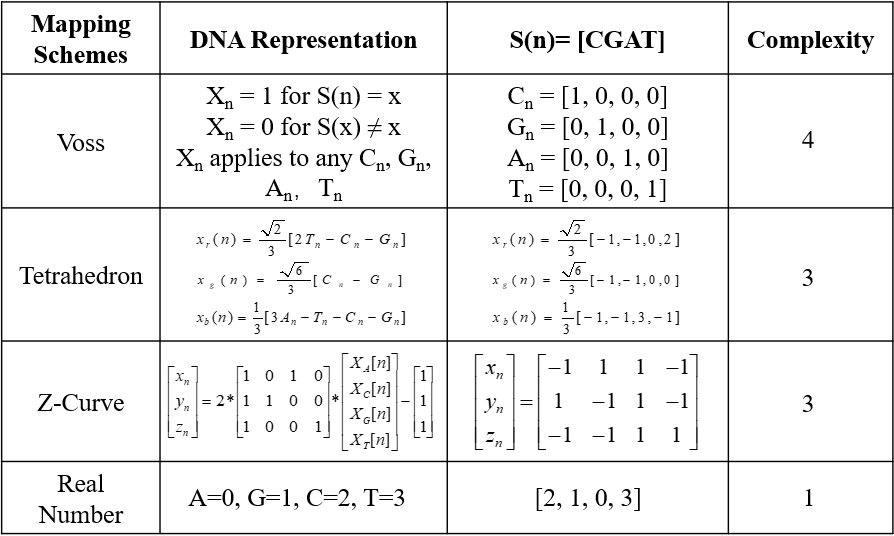
\includegraphics[width=\linewidth]{diff_mapping.png}
    \caption{Different Mapping Schemes Comparison}
    \label{fig1}
\end{figure}
~\\ \indent Voss mapping is a basic mapping scheme and tetrahedron mapping is a kind of dimension reduction of voss mapping. Z-curve mapping is a magical method which has excellent biological significance. And the real number mapping is a method that strives for computing efficiency but ignores part of practical value.

\section{Modeling}
\subsection{Power Spectrum and SNR}
\subsubsection{A New Mapping Scheme}
~\\\indent In order to digitize the DNA , we need use a sequences to expresses the DNA, we Let I = {A, T, G, C}, any DNA sequence of length N can be expressed as:
\begin{equation}
    S=\{S[n]\mid S[n]\in I, n=0,1,...,N-1\}
\end{equation}
~\\\indent That is, the symbol sequence S of A, C, T and G: S[0], S[1],..., S[n-1]. For any given n less than N, we use two sequences to record the n-th base. Concretely speaking, we use a[n]=0, b[n]=0 to express S[n]=A, we use a[n]=1, b[n]=0 to express S[n]=C, we use a[n]=0, b[n]=1 to express S[n]=T, and we use a[n]=1, b[n]=1 to express S[n]=G.\\
i.e.
\begin{equation}\label{mapping}
    a[n]=\begin{cases}
    1& \text{S[n]=C/G}\\
    0& \text{S[n]=A/T}
    \end{cases},\ \ \ \ 
    b[n]=\begin{cases}
    1& \text{S[n]=T/G}\\
    0& \text{S[n]=A/C}
    \end{cases}
\end{equation}

~\\
\subsubsection{Fourier Transform Analysis}
~\\\indent In order to study the characteristics of DNA coding sequences. Discrete Fourier transform(DFT) should be performed on coding sequences. But it's too complex to perform DFT on string. So, we can map DNA coding sequences to two 0-1 sequences through our mapping.
~\\ \indent Assuming that a given DNA sequence fragment is S=ACTGAGCT, the two generated 0-1 sequences can be divided into two groups using our mapping shown in euqation \ref{mapping}:
$$\begin{aligned}\{a[n]\}:\{0,1,0,1,0,1,1,0\} \\
\{b[n]\}:\{0,0,1,1,0,1,0,1\}
\end{aligned}$$ 
~\\ \indent For these two 0-1 sequences, we can easily  perform DFT of them through DFT formula:
\begin{equation}\label{DFT-formula}
    \begin{aligned} A[k]=\sum_{n=0}^{N-1}{a[n]e^{-j\frac{2\pi nk}{N}}},\ k=0,1,...,N-1\\
B[k]=\sum_{n=0}^{N-1}{b[n]e^{-j\frac{2\pi nk}{N}}},\ k=0,1,...,N-1
\end{aligned}
\end{equation}
~\\
\subsubsection{Calculating Power Spectrum and SNR}
~\\\indent The square power spectrum of the complex sequence P[k] and Q[k] was calculated and added to obtain the spectrum power sequence \{P[k]\} of the whole DNA sequence S:
\begin{equation}\label{power-spectrum}
    P[k]=|A[k]|^2+|B[k]|^2
\end{equation}
~\\ \indent The power spectrum curve of the exon sequence has a large peak at the frequency of k=N/3, while the intron has no similar peak. This statistical phenomenon is called the "triple periodicity of bases".
~\\ \indent The average value of the total power of DNA sequence S is:
\begin{equation}\label{power}
    \bar{E}=\frac{\sum_{k=0}^{N-1}{P[k]}}{N}
\end{equation}
~\\ \indent The ratio of the power spectrum value of DNA sequence at a specific position, i.e. k=N/3, to the average value of the total power spectrum of the whole sequence s is taken as the "signal-noise ratio"(SNR) of the DNA sequence:
\begin{equation}\label{SNR}
    R = \frac{P[\frac{N}{3}]}{\bar{E}}
\end{equation}
~\\ \indent The SNR of a DNA sequence not only indicates the relative height of Peak Value, but also reflects the strength of triple periodicity of coding or non coding sequence.
~\\ \indent The exons of DNA sequences usually satisfy that the SNR is higher than a properly selected threshold (such as 2), while introns generally will not have this property.
~\\
\subsection{Genes Detection}
~\\\indent As the SNR of the exon and the intron is obviously different, we can detect and predict all exons of a complete DNA sequence that has not been annotated by using this characteristic. At present, there are two kinds of gene recognition algorithms based on SNR, "Fixed length sliding window method" and "Moving sequence method". We applied our mapping scheme to these two widely used algorithms
\subsubsection{Fixed length sliding window method}
~\\\indent For a DNA sequence s and its indicator sequences a[n] and b[n], n=0,1,2,\ldots,N-1. Take the length M (usually taken as a multiple of 3, such as M = 99, 129, 255, 513, etc.) as the fixed window length.
~\\ \indent For any $(0\le n \le N-1)$, On the sequence fragment $[n-\frac{M-1}{2}, n + \frac{M+1}{2}]$ with length M centered on n (when n is close to both ends of the sequence, the actual effective length of the window may be less than M), do Discrete Fourier Transform (DFT) for 2 indicator sequences.
\begin{equation}\label{DFT-sequence1}
    \begin{aligned} 
    A[k]&=\sum_{i=n-\frac{M-1}{2}}^{n+\frac{M+1}{2}}{a[i]e^{-j\frac{2\pi ik}{N}}},\ k=0,1,...,M-1\\
    B[k]&=\sum_{i=n-\frac{M-1}{2}}^{n+\frac{M+1}{2}}{b[i]e^{-j\frac{2\pi ik}{N}}},\ k=0,1,...,M-1
\end{aligned}
\end{equation} 
~\\ \indent The total spectrum $p(n;\frac{M}{3})$ at $\frac{M}{3}$ is shown as below:
\begin{equation}\label{total-sp}
    P[\frac{M}{3}]=|A[\frac{M}{3}]|^2+|B[\frac{M}{3}]|^2\triangleq P(n;\frac{M}{3})
\end{equation}
~\\ \indent Finally, just normalize the frequency spectrum value $p(n;\frac{M}{3})$, n=0,1,2,...,N-1.

~\\
\subsubsection{Moving sequence method}
~\\\indent Let S be a known DNA sequence and its indicative sequence is a[n] and b[n], n=0,1,2,...N-1. For any $n(0<n\le N-1)$, n is usually a multiple of 3 and increases gradually. On a sequence fragment [0, n-1] with length n on the left of n, the corresponding subsequence of DNA sequence S is called the "mobile subsequence" of DNA sequence $S_{0\sim n-1}$. Do Discrete Fourier Transform (DFT) on two indicator sequences corresponding to the mobile sequence:
\begin{equation}\label{DFT-sequence2}
    \begin{aligned} 
    A[k]&=\sum_{i=0}^{n-1}{a[i]e^{-j\frac{2\pi ik}{M}}},\ k=0,1,...,M-1\\
    B[k]&=\sum_{i=0}^{n-1}{b[i]e^{-j\frac{2\pi ik}{M}}},\ k=0,1,...,M-1
\end{aligned}
\end{equation}
~\\ \indent Then, calculate the SNR of moving subsequence:
\begin{equation}\label{SNR-move}
    R[n]=\frac{P[\frac{n}{3}]}{\bar{E}[n]}=\frac{|A[\frac{n}{3}]|^2+|B[\frac{n}{3}]|^2}{\bar{E}[n]},
\end{equation}
where $\bar{E}$ is the average power spectrum $\bar{E}[n]=\frac{\sum_{k=0}^{n-1}{P[k]}}{n}$ of the moving subsequence S.

\section{Results}
After we built the model, we did some experiments to evaluate the effect of our model. We did the following experiments:
~\\\indent 1.Power spectrum and signal-noise ratio experiment of voss mapping, z-curve mapping, real number mapping, binary mapping.
~\\\indent 2.Compare and evaluate the experiment results of different mapping schemes.
~\\\indent 3.Evaluate the experiment results in genes detection using binary mapping.

\subsection{Power Spectrum and SNR}
~\\ \indent The following graphs is a comparison of different mapping schemes's results of a lot of experiments.
\begin{figure}[H]
    \centering
    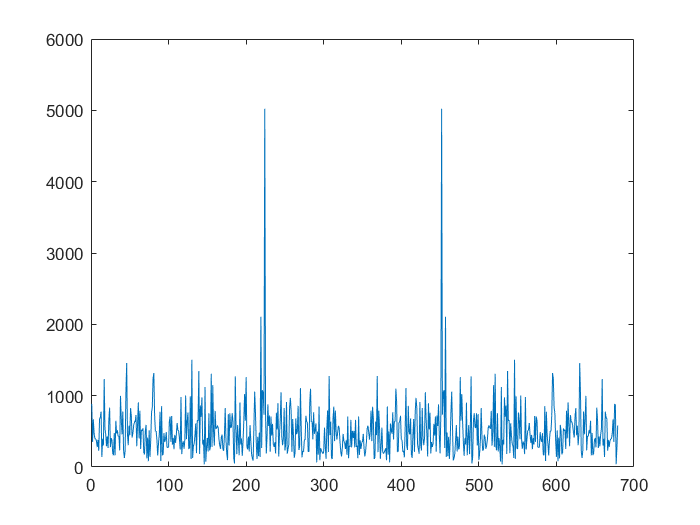
\includegraphics[width=\linewidth]{vossp.png}
    \caption{Voss mapping Power Spectrum}
    \label{vossp}
\end{figure}
~\\ \indent This is the result power spectrum graph of Voss mapping scheme, and its SNR is 7.3421. It can be seen from the figure that the power spectrum of Voss mapping has an obvious peak at $\frac{N}{3}$ and $\frac{2N}{3}$, indicating that the scheme conforms to the triple periodicity of bases.
\begin{figure}[H]
    \centering
    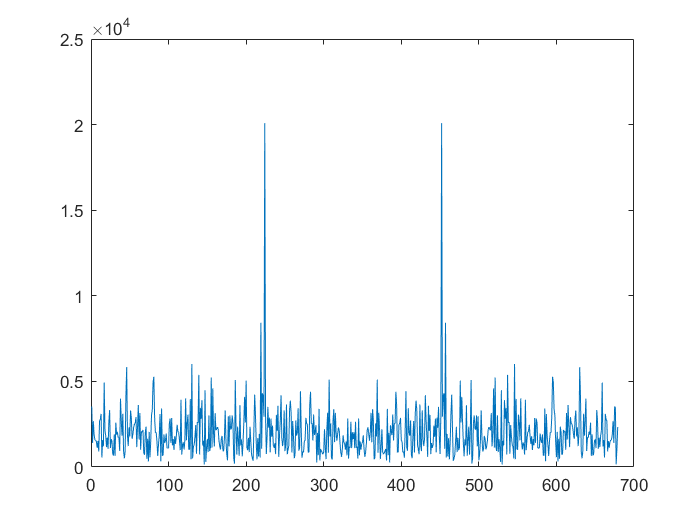
\includegraphics[width=\linewidth]{zcurvep.png}
    \caption{Z-curve mapping Power Spectrum}
    \label{zcurvep}
\end{figure}
~\\ \indent This is the result power spectrum graph of Z-curve mapping scheme, and its SNR is 9.7895. It can be seen from the figure that the power spectrum of Z-curve mapping has an obvious peak at $\frac{N}{3}$ and $\frac{2N}{3}$, indicating that the scheme conforms to the triple periodicity of bases. And Z-curve mapping obviously has a higher SNR, and the effect is excellent, mainly because the mapping is proposed from the biological principle, so the processing of bases is better.
\begin{figure}[H]
    \centering
    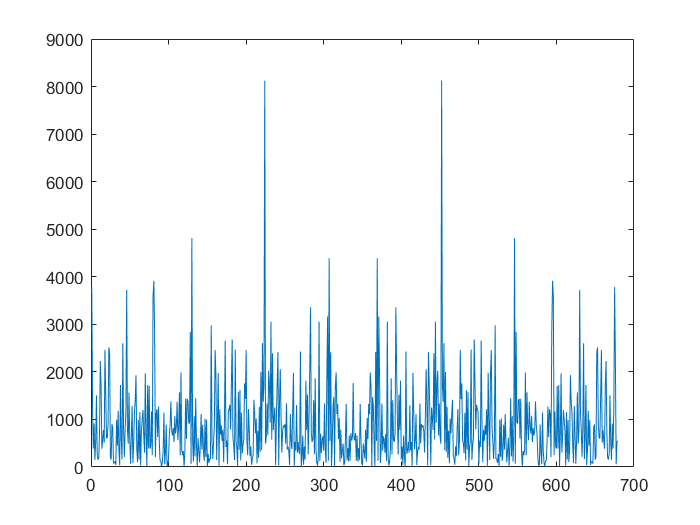
\includegraphics[width=\linewidth]{realp.png}
    \caption{Real mapping Power Spectrum}
    \label{realp}
\end{figure}
~\\ \indent This is the result power spectrum graph of Real mapping scheme, and its SNR is 3.2422. It can be seen from the figure that the power spectrum of Real mapping has an obvious peak at $\frac{N}{3}$ and $\frac{2N}{3}$, indicating that the scheme also conforms to the triple periodicity of bases. However, it can be clearly seen from the figure that the SNR value is not high, indicating that the noise of the mapping is too large, and it cannot display the triple periodicity of the base as well as the previous two mappings.
\begin{figure}[H]
    \centering
    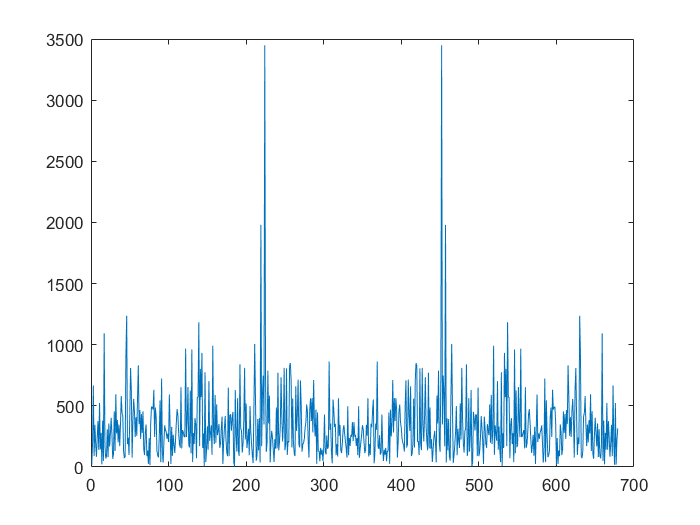
\includegraphics[width=\linewidth]{binaryp.png}
    \caption{Binary mapping Power Spectrum}
    \label{binaryp}
\end{figure}
~\\ \indent This is the result power spectrum graph of Binary mapping scheme, and its SNR is 5.8458. It can be seen from the figure that the power spectrum of our Binary mapping has an obvious peak at $\frac{N}{3}$ and $\frac{2N}{3}$, indicating that the scheme conforms to the triple periodicity of bases. And this mapping has a lower SNR than the real mapping, the effect is better, and the base three periodicity performance is more obvious.
% Please add the following required packages to your document preamble:
% \usepackage[table,xcdraw]{xcolor}
% If you use beamer only pass "xcolor=table" option, i.e. \documentclass[xcolor=table]{beamer}
~\\ \indent We implement the four schemes on 13 sequences of Human mtDNA, obtaining the following table that demonstrates our results, of which each row represents the performances of different mapping schemes on a particular sequence.
\begin{table}[H]\label{result1}
\scriptsize
\centering
\caption{Experiment Results}
\begin{tabular}{|c|c|c|c|c|}
\hline
{\color[HTML]{000000} SNR} & {\color[HTML]{000000} zcurve} & {\color[HTML]{000000} voss} & {\color[HTML]{000000} real} & {\color[HTML]{000000} binary} \\ \hline
NC\_012920\_1\_cds\_Seq1   & 16.0930                       & 12.0698                     & 8.3001                      & 10.6052                       \\ \hline
NC\_012920\_1\_cds\_Seq2   & 13.0857                       & 9.8143                      & 7.9654                      & 8.2060                        \\ \hline
NC\_012920\_1\_cds\_Seq3   & 32.6468                       & 24.4851                     & 10.3275                     & 20.8106                       \\ \hline
NC\_012920\_1\_cds\_Seq4   & 9.7895                        & 7.3421                      & 3.2422                      & 5.8458                        \\ \hline
NC\_012920\_1\_cds\_Seq5   & 1.4193                        & 1.0645                      & 1.1427                      & 1.3150                        \\ \hline
NC\_012920\_1\_cds\_Seq6   & 14.8370                       & 11.1278                     & 11.4896                     & 7.1190                        \\ \hline
NC\_012920\_1\_cds\_Seq7   & 5.3624                        & 4.0218                      & 2.0417                      & 3.6005                        \\ \hline
NC\_012920\_1\_cds\_Seq8   & 4.8821                        & 3.6615                      & 1.8931                      & 3.8906                        \\ \hline
NC\_012920\_1\_cds\_Seq9   & 7.5241                        & 5.6431                      & 3.8811                      & 4.8514                        \\ \hline
NC\_012920\_1\_cds\_Seq10  & 17.3332                       & 12.9999                     & 10.0151                     & 11.6665                       \\ \hline
NC\_012920\_1\_cds\_Seq11  & 30.5401                       & 22.9051                     & 14.3293                     & 20.0282                       \\ \hline
NC\_012920\_1\_cds\_Seq12  & 5.6000                        & 4.2000                      & 2.7081                      & 1.1264                        \\ \hline
NC\_012920\_1\_cds\_Seq13  & 18.5787                       & 13.9341                     & 4.4837                      & 15.5884                       \\ \hline
\end{tabular}
\end{table}
~\\\indent In terms of calculation, the main time to calculate the power spectrum and signal-noise ratio is spent on discrete fourier transform. Voss mapping requires four discrete fourier transforms, and Z-curve mapping requires three discrete fourier transforms, binary mapping requires two discrete fourier transforms, and real number mapping requires one discrete fourier transform. In terms of calculation speed, binary mapping is 2 times faster than Voss mapping and 1.5 times Z-curve mapping.
~\\\indent In terms of the final result, through analyzing the multiple sets of data obtained from our experiment, the real number mapping obtained signal-noise ratio is generally low, the experimental effect is not satisfactory. In most cases, it is worse a lot than binary mapping. The Z-curve mapping has the best experimental effect. And the results of binary mapping is as good as Voss mapping.
~\\\indent Although the real number mapping is the fastest mapping of the four mapping schemes, the signal-noise ratio of real number mapping is generally low. Most of DNA sequence fragments can't get a satisfactory result. Although the experimental effect of our binary mapping is not as perfect as Z-Curve, but our binary mapping can get the enough high SNR and the obvious triple periodicity with only $\frac{2}{3}$ time of Z-Curve mapping. Generally speaking, our binary mapping has such a good comprehensive effect.
\subsection{Genes Detection}
Our mapping method has achieved good results in calculation of power spectrum and SNR. Next, we use our binary mapping on the genes detection of all the sequences of Human mtDNA, and use two methods to evaluate our binary mapping scheme.
\subsubsection{Fixed length sliding window method}
~\\
\begin{figure}[H]
    \centering
    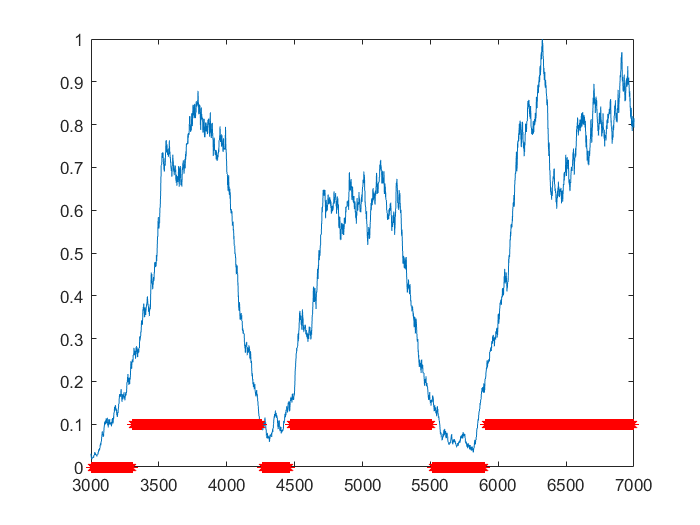
\includegraphics[width=\linewidth]{fixb.png}
    \caption{Binary mapping}
    \label{fixb}
\end{figure}
~\\\indent The upper red line in the figure represents the exon region, and the lower red line represents the intron region. As can be seen from the figure, the boundary between exons and introns is very obvious, and the two can be easily distinguished, indicating that our binary mapping has a good effect on gene recognition.
\begin{figure}[H]
    \centering
    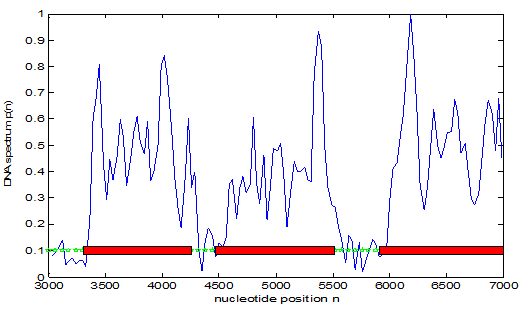
\includegraphics[width=\linewidth, height=0.75\linewidth]{fixv.png}
    \caption{Voss mapping}
    \label{fixv}
\end{figure}
~\\\indent Similar to the above results, the red line in the figure represents the exon region, and can be seen that Voss mapping can also clearly distinguish the two.
~\\\indent By analyzing the above two results, we can find that the results obtained by the two mapping methods are very similar, and both have good recognition results, which shows that our binary mapping can use the Fixed length sliding window method smoothly.
\subsubsection{Moving sequence method}
~\\
\begin{figure}[H]
    \centering
    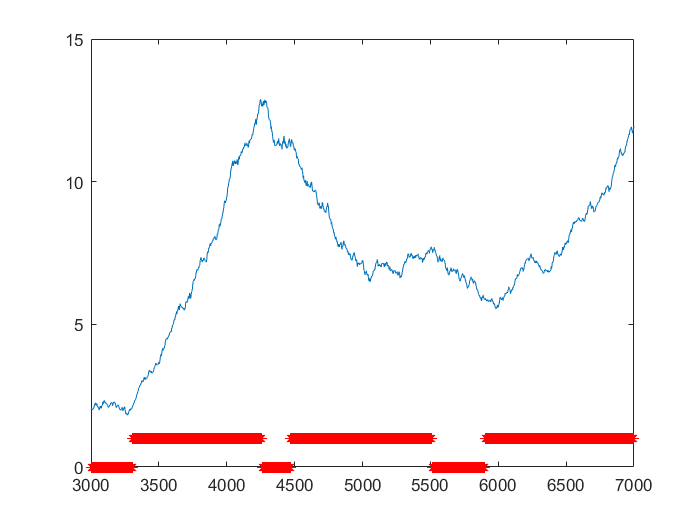
\includegraphics[width=\linewidth]{moveb.png}
    \caption{Binary mapping}
    \label{moveb}
\end{figure}
~\\\indent The upper red line in the figure represents the exon region, and the lower red line represents the intron region. As can be seen from the figure, We can relatively clearly distinguish two regions, indicating that our binary mapping has a good effect on gene recognition using Moving sequence method.
\begin{figure}[H]
    \centering
    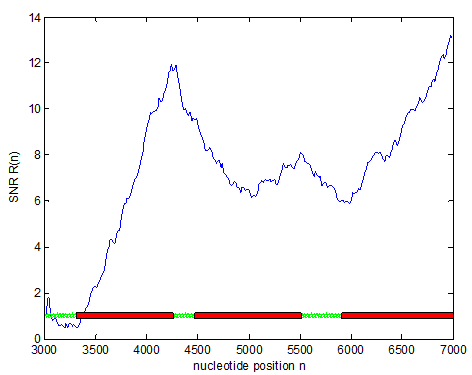
\includegraphics[width=0.9\linewidth]{movev.png}
    \caption{Voss mapping}
    \label{movev}
\end{figure}
~\\\indent The red line in the figure represents the exon region, and the green line represents the intron region. Similar to the above results, Voss mapping can also relatively clearly distinguish two regions.
~\\\indent By analyzing the above two results, we can find that the results obtained by the two mapping methods are very similar, and both have good recognition results, which shows that our binary mapping can use the moving sequence method smoothly.
~\\\indent Binary mapping can well support fixed length sliding window algorithm and moving sequence algorithm in genes detection. So we can use binary mapping to do genes detection and other related work.

\section{Conclusion}
In this article, we propose a new mapping scheme, which can map a DNA sequence into two numerical sequences, and then the sequence can be analyzed by the DSP method. By doing DFT on these two sequences, we can achieve the purpose of analyzing the original DNA sequence. 
~\\\indent Our team analyzed the power spectrum of different mapping schemes. Through comparison with different mapping schemes, we found that the binary mapping we proposed can well meet a series of requirements for DNA sequence analysis. A complete set of DNA sequence analysis methods including gene detection methods can be applied to our proposed binary mapping. Moreover, our binary mapping can also obtain better speed and close recognition results than Voss mapping. In theory, our binary mapping is twice as fast as the voss mapping.
~\\\indent In conclusion, our binary mapping is a well-performing method considering both computational efficiency and experimental results, and provides more choices for gene prediction.
\newpage
\nocite{*}
\bibliographystyle{IEEEtran}
\bibliography{DNA}
\end{document}
